\documentclass[a4paper]{article}

\usepackage[english]{babel}
\usepackage[utf8]{inputenc}
\usepackage{amsmath}
\usepackage{graphicx}
\usepackage{hyperref}
\usepackage[colorinlistoftodos]{todonotes}

\title{CS5011 Machine Learning Contest Report}

\author{Srikanth Prabala, EE12B053\\
		Rishiraj Surti, EE12B120\\
		Rahul Vadaga, EE12B122\\
		Team ID: 14
		}

\date{\today}

\begin{document}
\maketitle

\section{Algorithm}
Instead of developing new methods, we thought of implementing the existing classification algorithms and take the maximum likely class labels from the outputs.\\

We implemented the following algorithms:
\begin{itemize}
\item LibSVM, Gaussian, Polynomial, Sigmoid Kernels.
\item Sklearn SVM, Gaussian Kernel
\item KNN, k=7 
\item LDA
\item Neural Network (Backpropagation)
\item Bayes, Bernoulli and Multinomial
\end{itemize}

For the test data, we took the output which had a maximum vote among these algorithms.
To try something different, we thought of giving priorities. But that didn't work out well. So instead, we repeated the outputs of some of our algorithms. As an example, from our experience, Neural Network works better. So we just repeated its output twice. If NN gave a wrong output, others would take care. But if it is a correct one, we made sure it gets noticed. In this case as the input data is very large so we have used large number of hidden neurons which tries to capture the data correctly. The learning rate is kept low so that the function settles to a good optimum value. \\


We also came to conclusion that SVM with Gaussian kernel gave better F1 measure than others. So our prediction was that the data was some kind of mixture of Gaussians. As the f1 measure of other teams revolved around the value 0.6, we gauged that it could be a mixture of "highly overlapping" gaussians, impossible to seperate beyond a certain point. We tried to work around the same idea. 


\begin{figure}
\centering
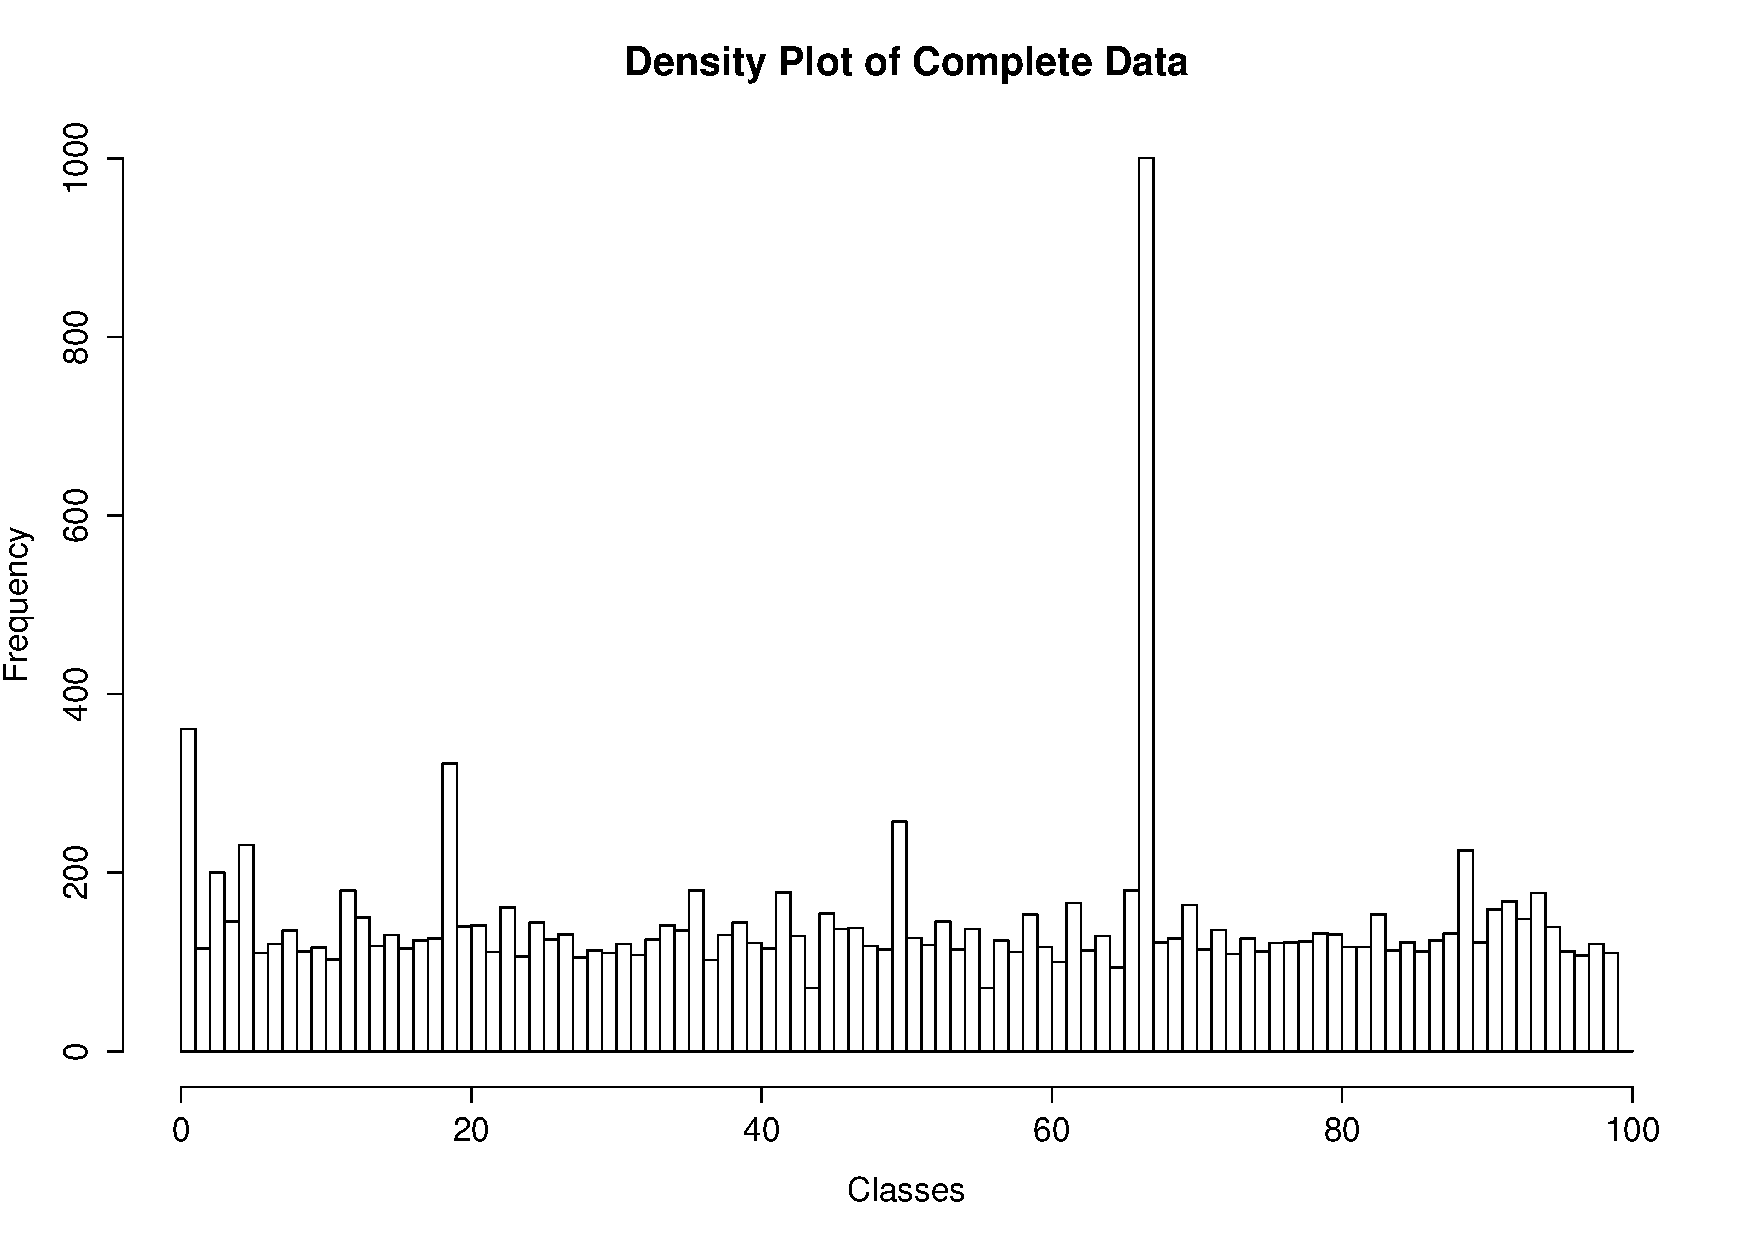
\includegraphics[width=1\textwidth]{../plots/CompleteData_targets.pdf}
\caption{\label{fig:data}}
\end{figure}

\section{Code}
We had a private Github repository to work for this contest.
The link to repo:\\ \href{https://github.com/rishirajsurti/ml_contest}{ml\_contest} \\
\href{https://github.com/rishirajsurti/ml_contest/graphs/contributors}{ml\_contest\_graphs}\\
Please mail me at rishirajsurti.iitm@gmail.com with your Github username to gain access to repo.
The file which generates the final output is "compare.py".
This has an array of output files of algorithms implemented and chooses the most likely label among these.


\end{document}
              